%%%%%%%%%%%%%%%%%%%%%%%%%%% asme2e.tex %%%%%%%%%%%%%%%%%%%%%%%%%%%%%%%
% Template for producing ASME-format articles using LaTeX            %
% Written by   Harry H. Cheng                                        %
%              Integration Engineering Laboratory                    %
%              Department of Mechanical and Aeronautical Engineering %
%              University of California                              %
%              Davis, CA 95616                                       %
%              Tel: (530) 752-5020 (office)                          %
%                   (530) 752-1028 (lab)                             %
%              Fax: (530) 752-4158                                   %
%              Email: hhcheng@ucdavis.edu                            %
%              WWW:   http://iel.ucdavis.edu/people/cheng.html       %
%              May 7, 1994                                           %
% Modified: February 16, 2001 by Harry H. Cheng                      %
% Modified: January  01, 2003 by Geoffrey R. Shiflett                %
% Use at your own risk, send complaints to /dev/null                 %
%%%%%%%%%%%%%%%%%%%%%%%%%%%%%%%%%%%%%%%%%%%%%%%%%%%%%%%%%%%%%%%%%%%%%%

%%% use twocolumn and 10pt options with the asme2e format
\documentclass[cleanfoot,cleanhead,twocolumn,10pt,notitlepage]{asme2e}
\special{papersize=8.5in,11in}

\usepackage{listings}
\usepackage{graphicx}
\usepackage{amsmath}
\lstset{
    breaklines=true, % break lines for files
    basicstyle=\scriptsize,
    numbers=left,
    showstringspaces=false,
    frame=l
}

%% The class has several options
%  onecolumn/twocolumn - format for one or two columns per page
%  10pt/11pt/12pt - use 10, 11, or 12 point font
%  oneside/twoside - format for oneside/twosided printing
%  final/draft - format for final/draft copy
%  cleanfoot - take out copyright info in footer leave page number
%  cleanhead - take out the conference banner on the title page
%  titlepage/notitlepage - put in titlepage or leave out titlepage
%  
%% The default is oneside, onecolumn, 10pt, final

%%% You need to remove 'DRAFT: ' in the title for the final submitted version.
\title{Computer Project \#2}

%%% first author
\author{Shaun Harris
    \affiliation{
	Department of Mechanical and Aerospace Engineering\\
	Utah State University \\
    Email: shaun.r.harris@gmail.com
    }
}


\begin{document}

\maketitle    

%%%%%%%%%%%%%%%%%%%%%%%%%%%%%%%%%%%%%%%%%%%%%%%%%%%%%%%%%%%%%%%%%%%%%%

\begin{abstract}
    {\it A Convection problem is calculated in this project.  Neglecting the diffusion terms, and setting density to one yields the governing equation of $\frac{\partial}{\partial x}\left( u \phi \right) + \frac{\partial}{\partial y} \left( v \phi \right) = 0$.  Having the domain of $0 \le x \le 1$ and $0 \le y \le 1$ and letting $u = v = 1$ we can implement the deferred correction method to solve the solution.  The solutions for $\beta = 0.0, 0.9, 1.0$ are shown.}
\end{abstract}

%%%%%%%%%%%%%%%%%%%%%%%%%%%%%%%%%%%%%%%%%%%%%%%%%%%%%%%%%%%%%%%%%%%%%%

\begin{nomenclature}
\entry{$u$}{Velocity in the x-direction}
\entry{$v$}{Velocity in the y-direction}
\entry{$\phi$}{General Parameter per unit mass}
\entry{$\phi^L$}{Lower order approximation of $\phi$}
\entry{$\phi^H$}{Higher order approximation of $\phi$}
\entry{$F_i$}{Flux coefficient on the $i$ face, ($n,e,s,$ or $w$)}
\entry{$a_i$}{Coefficient for final discretized equation on cell center $i$ using lower order approximation}
\entry{$\tilde{a_i}$}{Coefficient for final discretized equation on cell center $i$ using higher order approximation}
\entry{$\beta$}{Blending factor for deferred correction method}
\end{nomenclature}

%%%%%%%%%%%%%%%%%%%%%%%%%%%%%%%%%%%%%%%%%%%%%%%%%%%%%%%%%%%%%%%%%%%%%%

\section*{INTRODUCTION}

A convection of a step profile in a uniform incompressible flow is considered.  This problem neglects diffusion and sets density to one.  The governing equation now becomes like Eq. \ref{eq:gov}.

\begin{equation}
\begin{aligned}
\frac{\partial}{\partial x}\left( u \phi \right) + \frac{\partial}{\partial y} \left( v \phi \right) = 0
\label{eq:gov}
\end{aligned}
\end{equation}

This equation was altered using a numerical method and then applied to a system of equations.  The solution to the system of equations yielded the true values of $\phi$ for the convection problem.  

The boundary conditions were provided as shown in Eq. \ref{eq:BC}.  This provided for a more accurate convection problem.  

\begin{equation}
\begin{aligned}
\left.\phi\right|_{Left~Wall} &= 100 \\
\left.\phi\right|_{Bottom~Wall} &= 100 \\
\left. \frac{\partial \phi}{\partial x}\right|_{Right~Wall} &= 0 \\
\left. \frac{\partial \phi}{\partial y}\right|_{Top~Wall} &= 0
\label{eq:BC}
\end{aligned}
\end{equation}

The numerical method and results are shown in the next sections.
%%%%%%%%%%%%%%%%%%%%%%%%%%%%%%%%%%%%%%%%%%%%%%%%%%%%%%%%%%%%%%%%%%%%%%

\section*{NUMERICAL METHOD}

The following steps for followed to achieve a numerical method for this problem.  

\begin{enumerate}
\item Grid generation
\item Discretization of equations
\item Solution of equations
\end{enumerate}

To generate the grid, and formulation represented by Fig. \ref{fig:stencil} was generated.  This figure shows the point P and the corresponding neighbor cells N,E,S, and W.  

To discretize the grid the volume integral of Eq. \ref{eq:gov} over the cell volume P.  The discretization is shown in Eq. \ref{eq:disc}.

\begin{equation}
\begin{aligned}
\frac{\partial}{\partial x}\left( u \phi \right) &+ \frac{\partial}{\partial y} \left( v \phi \right) &= 0 \\
\iiint_V \frac{\partial}{\partial x}\left( u \phi \right)~dx~dy~dz &+ \iiint_V \frac{\partial}{\partial y} \left( v \phi \right)~dx~dy~dz &= 0 \\
(u\phi A)_e - (u\phi A)_w &+ (v\phi A)_n - (v\phi A)_s &=0\\
\text{Assume: } & A_e = A_w = A_n = A_s &= A \\
(u\phi)_e - (u\phi)_w &+ (v\phi)_n - (v\phi)_s &=0 \\
\label{eq:disc}
\end{aligned}
\end{equation}

In order to solve for the face values shown in the equation we needed to incorporate upwinding and central differencing schemes.  It was found that upwinding passed all the criteria and gave stable results, but yielded false diffusion results.  While central differencing gave semi-stable results but did not pass the transitivenesses criteria.  It did not account for the direction of the flow in the numerical analysis.  

Both of these solutions could be combined, however, and yield a deferred correction method.  These solutions were combined as shown in Eq. \ref{eq:combine}.  

\begin{equation}
\phi \approx \phi^L + \beta (\phi^H - \phi^L)
\label{eq:combine}
\end{equation}

Eq. \ref{eq:disc} and \ref{eq:combine} were combined to yield the final discretized equation in Eq. \ref{eq:discfinal}

\begin{equation}
\begin{aligned}
\phi_P = \frac{a_W\phi_W+a_S\phi_S}{a_P}-&\frac{\beta}{a_P}\left[ \tilde{a_P}\phi_P - \tilde{a_E}\phi_E-\tilde{a_W}\phi_W-\tilde{a_N}\phi_N-\tilde{a_S}\phi_S \right.\\ 
&+\left.a_P\phi_P+a_W\phi_W+a_S\phi_S \right]\\
\text{Where: }\\
&a_W = u\\
&a_E = 0\\
&a_S = v\\
&a_N = 0\\
&a_P = a_W + a_S\\
&\tilde{a_W} = \frac{u}{2}\\
&\tilde{a_E} = \frac{-u}{2}\\
&\tilde{a_S} = \frac{v}{2}\\
&\tilde{a_N} = \frac{-v}{2}\\
&\tilde{a_P} = \tilde{a_W} + \tilde{a_E} + \tilde{a_S} + \tilde{a_N}
\label{eq:discfinal}
\end{aligned}
\end{equation}

This discretized equation was then applied to the grid to generate a system of equations.  It was then iterated over until the solution fully converged.  The various solutions are shown below.




%%%%%%%%%%%%%%%%%%%%%%%%%%%%%%%%%%%%%%%%%%%%%%%%%%%%%%%%%%%%%%%%%%%%%%

\section*{RESULTS}

The diagonal of the solution $\phi$ is shown in Fig. \ref{fig:be0}, \ref{fig:be09}, \ref{fig:be1}, \ref{fig:40X40}, and \ref{fig:contour}.  

Fig. \ref{fig:be0} shows the solution for total upwinding.  This is as if we did not implement any deferred correction method.  It can be seen that the upwinding yielding undesired diffusion around the middle section.  It was more noticeable for the coarser grids.  

Fig. \ref{fig:be09} shows the solution for the deferred correction method.  It can be seen that this has noticeably less diffusion along the middle line.  As we get more refined mesh we find that it gets closer and closer to the exact solution.  Thus, the artificial diffusion is minimized by both having a finer mesh, and by increasing the $\beta$ value.  

Fig. \ref{fig:be1} shows the solution for the central differencing approximation.  We can see that it yields the most accurate results for no artificial diffusion.  But it should be remembered that this scheme does not pass all the criteria for convection-diffusion solution.  The solution here may not be accurate if diffusion is involved.

Fig. \ref{fig:40X40} shows the solution for the finest grid for all the values of $\beta$.  We can easily see how the closer the $\beta$ value gets to one the closer the solution gets to the exact solution.  

Fig. \ref{fig:contour} shows the contour plot of the finest grid with a blending factor $\beta = 1.0$.  


%%%%%%%%%%%%%%%%%%%%%%%%%%%%%%%%%%%%%%%%%%%%%%%%%%%%%%%%%%%%%%%%%%%%%%

\section*{CONCLUSION}

The numerical method for approximating a convection problem has been shown here.  The solution of $\phi$ is shown for various values of $\beta$ for the deffered correction method. The artificial diffusion presented in the solution can be minimized by refining the grid, and by increasing the $\beta$ value using the deferred correction method.  


%%%%%%%%%%%%%%%%%%%%%%%%%%%%%%%%%%%%%%%%%%%%%%%%%%%%%%%%%%%%%%%%%%%%%%

%\bibliographystyle{asmems4}
%\bibliography{asme2e}

%%%%%%%%%%%%%%%%%%%%%%%%%%%%%%%%%%%%%%%%%%%%%%%%%%%%%%%%%%%%%%%%%%%%%%

%\section*{FIGURES}

\begin{figure}[t]
\begin{center}
    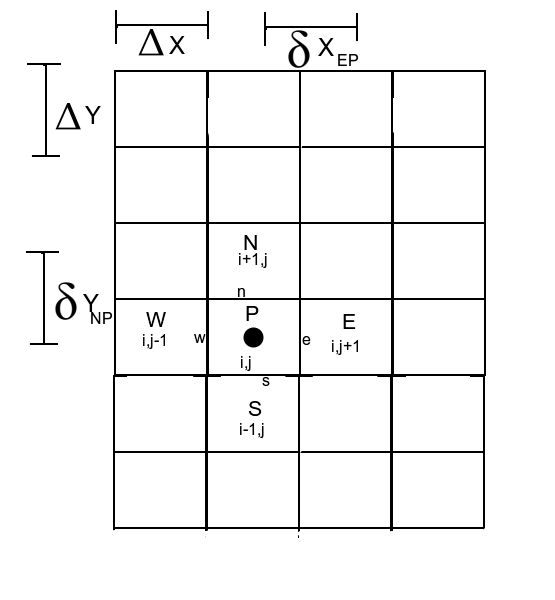
\includegraphics[width=\linewidth]{Stencil.png}
    \caption{REPRESENTATION OF STENCIL FOR GRID GENERATION}
    \label{fig:stencil}
\end{center}
\end{figure}

\begin{figure}[t]
\begin{center}
    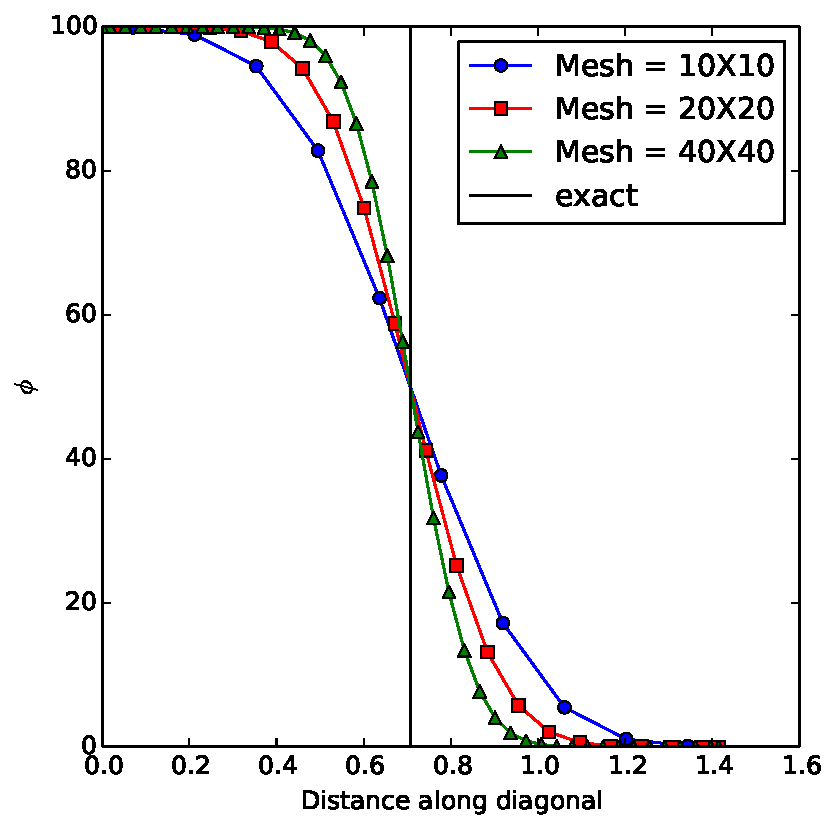
\includegraphics[width=\linewidth]{../Project2_code/Beta/Beta0/lines.pdf}
    \caption{DIAGONAL OF $\beta=0$ UPWINDING}
    \label{fig:be0}
\end{center}
\end{figure}

\begin{figure}[t]
\begin{center}
    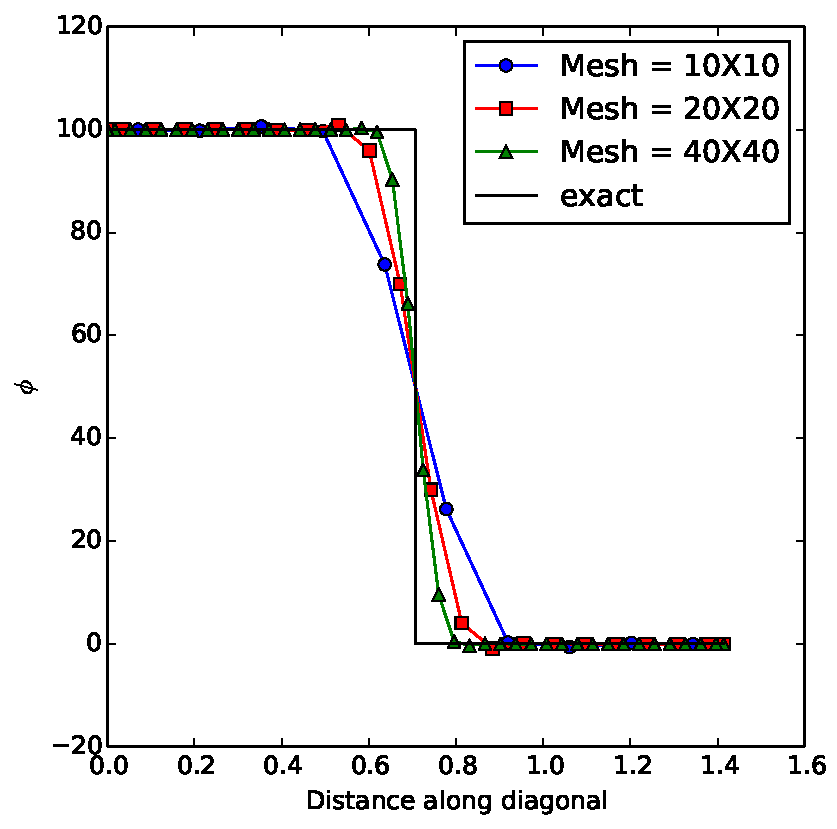
\includegraphics[width=\linewidth]{../Project2_code/Beta/Beta0_9/lines.pdf}
    \caption{DIAGONAL OF $\beta=0.9$ DEFERRED CORRECTION METHOD}
    \label{fig:be09}
\end{center}
\end{figure}

\begin{figure}[t]
\begin{center}
    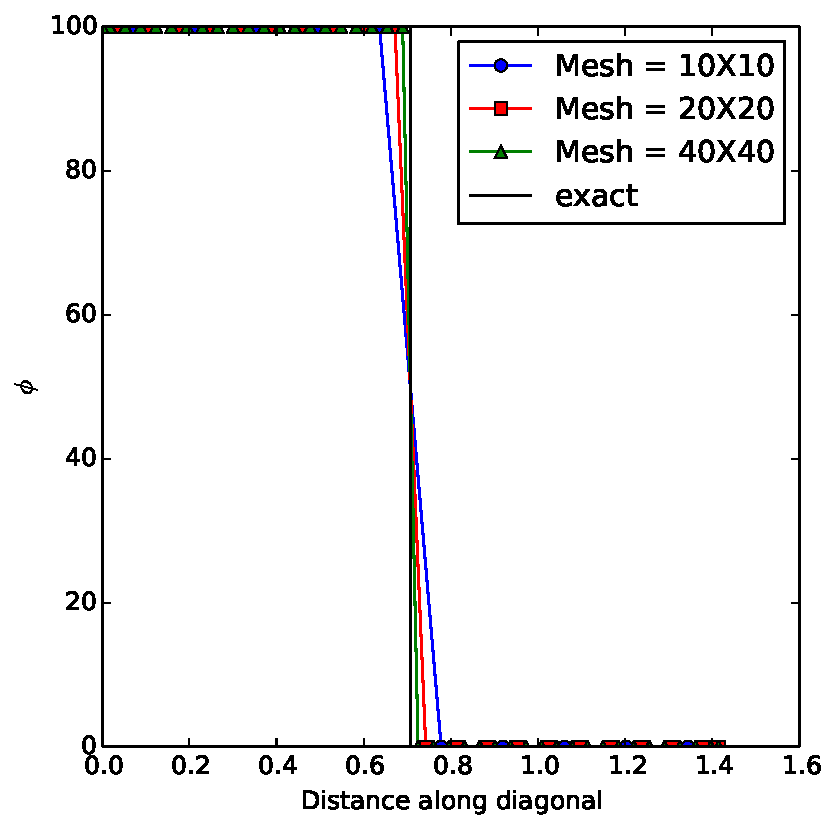
\includegraphics[width=\linewidth]{../Project2_code/Beta/Beta1/lines.pdf}
    \caption{DIAGONAL OF $\beta=1.$ CENTRAL DIFFERENCING}
    \label{fig:be1}
\end{center}
\end{figure}

\begin{figure}[t]
\begin{center}
    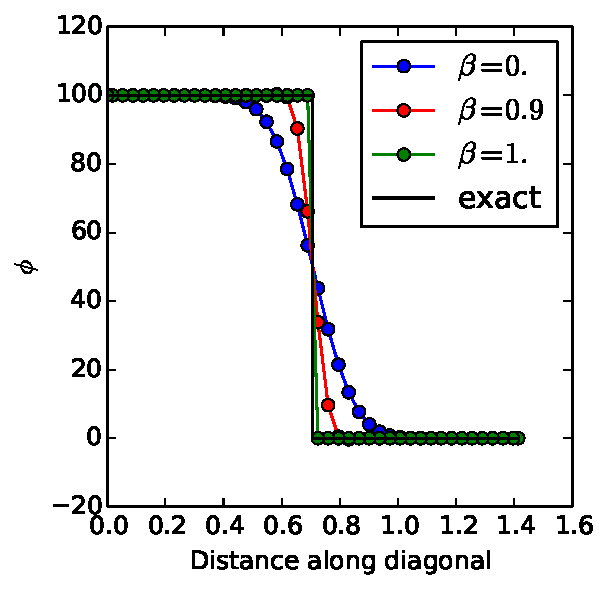
\includegraphics[width=\linewidth]{../Project2_code/Mesh/Mesh_40/lines.pdf}
    \caption{DIAGONAL OF 40X40 MESH DENSITY}
    \label{fig:40X40}
\end{center}
\end{figure}

\begin{figure}[t]
\begin{center}
    \includegraphics[width=\linewidth]{../Project2_code/output/Phi.pdf}
    \caption{CONTOUR PLOT OF PHI FOR MESH 40X40 AND $\beta = 1.$}
    \label{fig:contour}
\end{center}
\end{figure}
%%%%%%%%%%%%%%%%%%%%%%%%%%%%%%%%%%%%%%%%%%%%%%%%%%%%%%%%%%%%%%%%%%%%%%
\clearpage

\appendix

\section*{Appendix A: Code}

\lstinputlisting[language=Fortran]{../Project2_code/Project2.f90}



\end{document}
